\documentclass[10pt,a4paper,twocolumn]{article}
\usepackage[a4paper,left=2.25cm,right=2.25cm,top=2.0cm,bottom=2.1cm,columnsep=0.65cm]{geometry}
\usepackage[T1]{fontenc}
\usepackage[utf8]{inputenc}
\usepackage{newtxtext,newtxmath,microtype}
\renewcommand{\ttdefault}{cmtt}
\DeclareRobustCommand{\ttfamily}{\fontencoding{OT1}\fontfamily{cmtt}\selectfont}
\usepackage{graphicx,booktabs,amsmath,array,xcolor,url,natbib,tikz}
\usetikzlibrary{arrows.meta,positioning}
\usepackage[font=small,labelfont=bf]{caption}
\usepackage[breaklinks=true,hidelinks]{hyperref}
\definecolor{revision}{HTML}{B00020}
\definecolor{inkblue}{HTML}{185B83}
\newcommand{\rev}[2]{\par\smallskip\noindent\begin{minipage}{\linewidth}\color{revision}\footnotesize\textbf{REVISION #1.} #2\end{minipage}\par\smallskip}
\newcommand{\nd}{\texttt{non\_distinct}}
\newcommand{\wt}{\textsc{WorkTrace}}
\newcommand{\src}[1]{\path{#1}}
\setlength{\parindent}{1em}
\setlength{\parskip}{0pt}
\setlength{\textfloatsep}{10pt plus 2pt minus 2pt}
\setlength{\floatsep}{8pt plus 2pt minus 2pt}
\setlength{\intextsep}{9pt plus 2pt minus 2pt}
\renewcommand{\topfraction}{0.93}
\renewcommand{\bottomfraction}{0.85}
\renewcommand{\textfraction}{0.06}
\renewcommand{\floatpagefraction}{0.75}
\setcounter{topnumber}{3}
\setcounter{totalnumber}{5}
\setlength{\emergencystretch}{1em}
\title{\textbf{WorkTrace: Reconstructing and Comparing\\Work Progression in Coding Agents}}
\author{Anonymous working manuscript}
\date{Annotated research draft --- 26 October 2026}
\begin{document}
\maketitle
\begin{abstract}
Coding-agent evaluations summarize final task success and computational effort, leaving the organization of that effort difficult to compare. We present \wt, a framework that relates tool operations to work targets, inferred code states, and earlier evidence. It combines an object-progression view of investigation with a code-version view of revision and verification, and aggregates traces into comparative patterns. We report current results from two complementary panels: 6,300 runs of three models under a common harness and 6,000 runs of one model under three harnesses. The saved analyses reveal two principal observations. First, models differ in verification placement: Gemini concentrates checks on the final inferred version, whereas Luna and Terra distribute fewer checks more evenly across versions. Second, harnesses exhibit different revisit structures despite similar exact-repeat rates. Pilot semantic labels contextualize these observations but do not establish causal utility. We describe the framework, compare systems, and distinguish the supported structural observations from claims about oververification, overexploration, and removable work that require further validation.
\end{abstract}\par\medskip
\noindent\textit{Draft status.} All numerical results come from existing repository artifacts. No new agent experiments or human annotations were performed for this manuscript. Red text contains editorial improvement notes, separate from the proposed scientific claims.
\rev{01}{Regenerate the fact and graph outputs after the audited state/write fixes. Independent human validation is pending. The two abstract observations are provisional leads; do not promote them to verified mechanisms or ``overthinking'' without additional evidence.}

\section{Introduction}
Language-model coding agents solve issues through repository inspection, implementation, and execution. Two agents may reach the same outcome through different processes: one may revise a small region and repeatedly test it, while another may inspect many targets before implementing a patch. Success, token consumption, and call counts expose the amount of work but leave its organization implicit.

Understanding that organization matters for comparing models and agent harnesses. A higher revisit rate can indicate incremental inspection, recovery from an unsuccessful approach, or reconstruction of context. A long verification phase can check additional properties or repeat evidence already obtained. Interpreting these behaviors requires connecting operations to the state and purpose of surrounding work.

Structural analysis offers a precedent. TRACE decomposes answer-bearing reasoning, reconstructs progression graphs, and connects induced patterns to utility tracing and a stopping case study \citep{trace}. Coding-agent traces introduce changing external states, heterogeneous observation scopes, and support scripts alongside implementation changes. A representation must preserve the relationship between investigation, code changes, and evidence.

We introduce \wt\ for this comparative analysis. Its purpose is to explain how work unfolds. Candidate redundancy is one diagnostic within the framework, alongside exploration, refinement, recovery, and verification. We address three questions:
\begin{itemize}
\setlength{\itemsep}{1pt}\setlength{\topsep}{3pt}
\item \textbf{RQ1:} How can heterogeneous operations be represented as comparable work progressions?
\item \textbf{RQ2:} What structural differences appear across models under a common harness and across harnesses with a fixed model?
\item \textbf{RQ3:} Which conclusions require structural information, and what would establish their practical utility?
\end{itemize}
Our current observations concern \emph{final-version verification concentration} and \emph{harness-dependent revisit structure}. They motivate an explanatory study without presupposing that extended work is wasteful. They do not establish that particular checks or searches can safely be removed.
\rev{02}{State the explanation and decision enabled by each finding. The eventual contribution must exceed transferring TRACE's layout or observing that repetition differs from redundancy. Discover patterns on exploratory tasks and confirm the principal findings on fresh tasks.}

\section{Related Work}
\paragraph{Structural trajectory analysis.}
TRACE studies answer progression in reasoning traces \citep{trace}. Software-agent trajectory analysis examines thought--action--result relationships and recurring sequences \citep{bouzenia}. \wt\ extends this analytical direction by relating target visits to inferred implementation versions. Its intended contribution is a comparative account of changing work states and evidence, beyond an additional taxonomy alone.
\paragraph{Redundancy and efficiency.}
RedundancyBench evaluates redundant-step localization, categories, and supporting-evidence retrieval \citep{redundancybench}. Its annotation and component-evaluation procedures offer useful validation precedents. AgentDiet compresses agent histories \citep{agentdiet}; TRIM uses repair trajectories to minimize unnecessary final-patch edits \citep{trim}. Work organization, history compressibility, evidence novelty, patch minimality, and safe action removal require different evaluations.
\paragraph{Interaction.}
SWE-TaskFlow varies the interaction layer of verified tasks \citep{taskflow}. Such settings can test adaptation to new instructions. The present comparisons use the saved panels below and do not establish a controlled effect of user interaction.
\rev{03}{Complete claim-level positioning against these works. Credit adapted evidence/annotation procedures from RedundancyBench while retaining the software-work ontology. A redundancy-detector leaderboard would not establish this paper's intended explanatory contribution.}

\section{Benchmarking Agent Work}
\subsection{Comparison Panels}
\paragraph{Cross-model panel.}
The JetBrains-derived analysis contains 6,300 runs: three models, 700 tasks, and three runs per task--model pair under mini-swe-agent. Identifiers follow the stored metadata: Gemini 3.7 Flash, GPT-5.6 Luna, and GPT-5.6 Terra. The fact table contains 188,609 operations; gold-patch metadata is available for 93.9\% of runs. Table~\ref{tab:model} reports saved benchmark results.
\paragraph{Cross-harness panel.}
Open-SWE-Traces v1.2 supplies Qwen3.8-27B runs under mini-swe-agent, OpenHands, and SWE-agent \citep{openswe}. The sample contains 2,000 task IDs attempted by all harnesses, with one selected run per task--harness pair: 6,000 runs and 370,992 operations. Tasks originate from SWE-rebench-V2 and Scale-SWE in the stored release. Table~\ref{tab:harness} reports the saved results.
\begin{table*}[t]
\centering\small\setlength{\tabcolsep}{6pt}
\begin{tabular}{lrrrrr}
\toprule
Model & Resolve (\%) & Calls/run & Input tokens (M) & Exact repeats (\%) & Object revisits (\%)\\
\midrule
Gemini 3.7 Flash & 60.0 & 53.1 & 3.34 & 2.21 [2.08, 2.35] & 21.1\\
GPT-5.6 Luna & 50.0 & 17.6 & 0.25 & 0.02 [0.00, 0.03] & 11.1\\
GPT-5.6 Terra & 54.2 & 19.0 & 0.24 & 0.05 [0.03, 0.07] & 9.4\\
\bottomrule
\end{tabular}
\caption{Cross-model benchmark: 2,100 runs per model and 700 matched tasks under mini-swe-agent. Exact-repeat and revisit rates are means of per-run rates. Brackets reproduce task-bootstrap 95\% intervals for exact repeats; rounding does not imply a zero lower bound.}
\label{tab:model}
\end{table*}
\begin{table*}[t]
\centering\small\setlength{\tabcolsep}{4pt}
\begin{tabular}{lrrrrr}
\toprule
Harness & Resolve (\%) & Calls/run & Assistant text (k chars) & Exact repeats (\%) & Object revisits (\%)\\
\midrule
mini-swe-agent & 57.1 & 51.8 & 110.6 & 0.20 [0.14, 0.28] & 19.3 [18.9, 19.7]\\
OpenHands & 51.0 & 66.2 & 149.2 & 0.18 [0.16, 0.21] & 33.5 [33.0, 33.9]\\
SWE-agent & 54.5 & 67.5 & 258.1 & 0.20 [0.17, 0.23] & 30.9 [30.4, 31.3]\\
\bottomrule
\end{tabular}
\caption{Cross-harness benchmark: Qwen3.8-27B on the same 2,000 tasks. Exact repeats are run means; revisits are pooled operation rates, following the source table. Brackets are task-bootstrap 95\% intervals. Characters are recorded proxies, not tokens or monetary costs.}
\label{tab:harness}
\end{table*}
These panels answer conditional questions about models under one harness and harnesses for one model. Their task populations differ; they are not a fully crossed experiment and cannot be pooled to estimate model--harness interactions. Comparisons concern the released configurations rather than an isolated training or architectural effect.

\subsection{Pilots and Statistical Units}
The JetBrains semantic pilot contains 50 runs from 17 tasks and 1,432 operations: 789 Gemini, 315 Luna, and 328 Terra. One of 51 possible task--model combinations is absent because the sample was truncated to 50 runs. A second pilot contains 20 Open-SWE tasks across three harnesses, giving 60 runs and 4,018 operations. Every pilot operation has a stored primary label.

The primary annotator is recorded as DeepSeek-V4.1-Flash through the configured endpoint. GLM-5.3-Flash and three temperature-0.7 primary-model samples provide stability checks on 425 JetBrains items. Larger label shards exist, but the semantic results here use the explicitly defined pilots; partial scale labels are not pooled into a completed population study.

Saved intervals generally resample tasks, preserving associated runs and operations. The cross-model benchmark uses 300 bootstrap replicates; most v2 graph/pilot analyses use 1,000. We preserve the saved estimands and do not interpret overlapping intervals as equivalence. Return analysis uses task-clustered generalized estimating equations (GEE).
\rev{04}{Add paired differences with intervals for the main comparisons and harmonize run-mean versus pooled revisit rates. Identify source conditions/settings and missing-result categories. JetBrains metadata records 4,198 missing results: distinguish expected terminal omissions from genuinely missing observations before claiming complete logs.}

\section{The WorkTrace Framework}
\begin{figure*}[t]
\centering
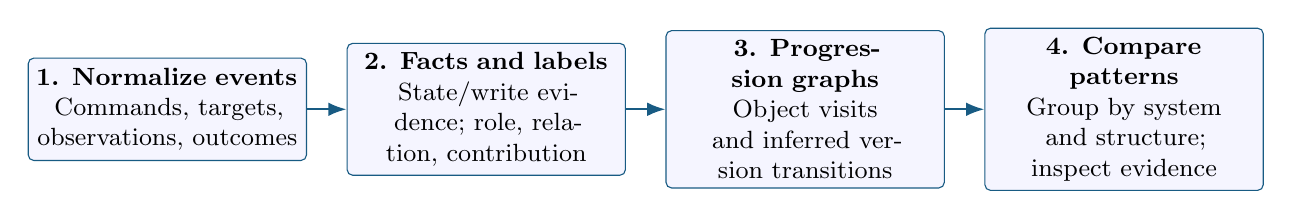
\begin{tikzpicture}[>=Latex,stage/.style={draw=inkblue,rounded corners=2pt,fill=blue!4,text width=3.3cm,align=center,minimum height=1.3cm,font=\small}]
\node[stage] (a) at (0,0) {\textbf{1. Normalize events}\\Commands, targets, observations, outcomes};
\node[stage] (b) at (4.05,0) {\textbf{2. Facts and labels}\\State/write evidence; role, relation, contribution};
\node[stage] (c) at (8.1,0) {\textbf{3. Progression graphs}\\Object visits and inferred version transitions};
\node[stage] (d) at (12.15,0) {\textbf{4. Compare patterns}\\Group by system and structure; inspect evidence};
\draw[->,thick,inkblue] (a)--(b);\draw[->,thick,inkblue] (b)--(c);\draw[->,thick,inkblue] (c)--(d);
\end{tikzpicture}
\caption{\wt\ pipeline. The graph views share operation IDs, enabling investigation to be inspected alongside implementation and verification. Current patterns are coordinate-aligned aggregates, not learned graph clusters or causal models.}
\label{fig:pipeline}
\end{figure*}
\subsection{Stage 1: Operation Normalization}
Operations record run/turn IDs, the agent message, invocation, observation, and available execution outcome. The parser splits shell chains for analysis while retaining the native tool call as the observed unit. It assigns read, search, edit, revert, run, probe, submit, or other kinds and identifies a main object. Mixed operations preserve constituent kinds.

Read objects commonly normalize to file paths; other objects can be commands or tool targets. These practical identifiers do not yet guarantee semantic equivalence across interfaces. Output normalization removes selected volatile fields for execution-like operations while preserving read content. Exact repetition requires normalized command and output-hash agreement.

\subsection{Stage 2: Facts and Evidence-Linked Labels}
For each operation, \wt\ retrieves the latest same-object operation and the latest same-kind operation with matching usable output. Short or explicitly truncated outputs are excluded from output-candidate retrieval. Facts describe output agreement and whether the object or code may have changed since a candidate.

Semantic annotation separates \emph{role} (e.g., explore, verify, revise), \emph{relation} (unmatched, revisits, reproduces, uncertain), and \emph{contribution} (distinct, non-distinct, uncertain). Labels cite operations and provide short rationales. For mixed operations, any distinct component makes the whole operation distinct.

The evidence validator restricts matched references to retrieved candidates and requires current and matched references for reproduces or \nd. An unmatched operation therefore cannot receive an accepted \nd\ label. Candidate-redundancy rates are reported under this restriction, rather than as a census of unnecessary work.
\rev{05}{Audit retrieval recall and allow valid evidence outside the two candidates. The unmatched-distinct skip check is constrained by the label rules; it cannot independently establish usefulness. Keep rule assignments separate from LLM annotations and preserve uncertain evidence.}

\subsection{Stage 3: Two Progression Views}
\paragraph{Object progression.}
Nodes represent targets and edges represent operations moving from the previous target to the current one. Immediate repeats form self-loops; later returns form back edges. A target can include purpose, but free-text purpose variation makes exact recurrence sparse. Existing analyses therefore use the object-only view as primary and retain purpose as supporting annotation.

For a return to target $u$ at operation $t$, with preceding visit $t'$, the detour count is
\begin{equation}
k_t=\left|\{u_j:t'<j<t\}\setminus\{u\}\right|.
\end{equation}
It counts intervening distinct targets, not distinct hypotheses or alternative solutions.

\paragraph{Code-version progression.}
Nodes represent inferred repository states. Recognized writes create provisional versions; unknown writes can create uncertain versions. Recognized restorations and content observations can map work back to earlier nodes. Non-writing execution attaches as a verification self-loop, except for detected read-only inline inspections. Edges describe initial moves, revisions, revisions after failures, backtracks, and no-ops.

The implementation calls a revision after a failed check \texttt{correct}. This rule label describes temporal context; it does not certify a correct patch. Final resolved status comes from the dataset, while intermediate versions have no independent correctness oracle.

Our primary figures exclude writes confined to inferred support files from implementation versions. Support candidates use file history and final submission metadata. This is a retrospective descriptive view, not an online estimator. Every-write and known-write-only variants are retained for sensitivity analysis.
\rev{06}{Fix status-based false identity, branch switches, incomplete mutation paths, and unknown effects. Failed restores and matching clipped diffs must not establish state equality. Recompute all downstream summaries; separate hindsight-based support hints from facts available online.}

\subsection{Stage 4: Pattern Aggregation}
Version graphs align by order and row: new versions advance horizontally and a new path after a backtrack advances vertically. Runs group by model and inferred version count. Node/edge weights record presence across runs; loops report mean verification operations. The saved figures prune components below 30\% presence and display groups of at least 20 runs.

Figure~\ref{fig:patterns} redraws saved four-version aggregates. Conditioning on version count controls one structural attribute but also selects on a trajectory outcome; these are illustrative slices, not unconditional model effects. Saved cross-harness aggregate version figures are not yet available.
\rev{07}{Test alignment/grouping/pruning sensitivity and report unpruned backtrack frequencies. A linear-looking aggregate can result from filtering or coordinate alignment. Validate each structural distinction before using it to explain system behavior.}

\section{Comparative Findings}
\subsection{Observation I: Verification Placement}
The support-excluded reconstruction yields mean inferred version counts of 4.78 for Gemini, 2.61 for Luna, and 2.59 for Terra. Recognized backtracks occur in 3.7\%, 0.2\%, and 0.7\% of runs. Recovered implementation trajectories are predominantly linear under these rules, which does not prove that an agent considered only one internal approach.
\begin{figure}[t]
\centering\includegraphics[width=\columnwidth]{images/verification.pdf}
\caption{Verification placement in runs with at least two inferred versions: 1,722 Gemini, 1,514 Luna, and 1,459 Terra. Earlier-version values first average within each run. Bars reproduce saved task-bootstrap 95\% intervals under the support-excluded reconstruction.}
\label{fig:verification}
\end{figure}
Gemini has 3.20 [3.01, 3.40] verification operations on the final inferred version versus 0.71 [0.63, 0.80] per earlier version. Corresponding values are 0.39 versus 0.46 for Luna and 0.47 versus 0.54 for Terra (Figure~\ref{fig:verification}). The final version receives 54.5\% of verification for Gemini and approximately 32\% for each GPT model in this selected population.
\begin{figure}[t]
\centering\includegraphics[width=\columnwidth]{images/patterns_four_versions.pdf}
\caption{Saved four-version aggregates redrawn without changing results. Nodes are inferred versions; percentages below show presence, blue self-loops show mean verification operations, and dashed rings mark frequently final coordinates. Arrows show dominant retained forward moves; components below 30\% presence are pruned. No intermediate correctness is marked.}
\label{fig:patterns}
\end{figure}

\paragraph{What comprises the final checks?}
Reconciliation compares each Gemini final-version check with earlier checks on that inferred version. Across 2,100 runs, 91.9\% [90.8, 93.0] use a different command, 1.9\% [1.5, 2.3] are identical command/output reruns, and 6.2\% use the same command with different output. The first check is different-command by definition. Approximately 95\% of multi-version runs have no identical rerun on the final version.

Rough command subtyping identifies suites, inline scripts, other test files, builds, and lint/type checks. This establishes heterogeneous command syntax, not necessarily distinct properties checked. In the 16-run Gemini pilot, 40 checks attach to final versions; 33 of 36 different-command checks are labeled distinct and three uncertain. One identical-rerun label contradicts the audited intervening facts, illustrating the need for independent semantic validation.

\paragraph{Interpretation.}
The representation localizes a difference that call counts cannot specify: Gemini's execution work accumulates before implementation and on the terminal inferred state, while Luna and Terra attach fewer checks throughout their version chains. This motivates a hypothesis about transitions from diagnostic checking to assurance. It does not yet establish expanded coverage, adequate confidence, or excessive verification.
\rev{08}{First phenomenon candidate: extract test/property scope and relevant-state dependencies, then separate diagnostic, change-validation, and additional-property checks. Account for length, version count, and unequal opportunity for final-state verification. Do not equate the final version with the first correct version or transfer TRACE's correctness-based interpretation without an oracle.}

\subsection{Observation II: Harness Revisit Patterns}
With Qwen fixed on matched tasks, exact-repeat run means are similar in magnitude: 0.20\%, 0.18\%, and 0.20\% for mini-swe-agent, OpenHands, and SWE-agent. Pooled object revisits span 19.3\% to 33.5\%, and calls range from 51.8 to 67.5 (Table~\ref{tab:harness}). These descriptive comparisons do not constitute an equivalence test.

Reads, searches, and edits comprise 30.5\%, 21.3\%, and 12.0\% of mini-swe-agent operations; 23.8\%, 19.7\%, and 23.4\% for OpenHands; and 26.8\%, 18.6\%, and 18.4\% for SWE-agent. Similar exact-repeat statistics thus coexist with different observed distributions of work.

Some revisit differences are representational. Structured editor views reuse file identifiers, whereas shell commands express separate ranges or search contexts. Current main-object extraction does not fully resolve this mismatch. The result is a difference in observed revisit structure; fragmented investigation, useful incremental inspection, and context reconstruction remain competing explanations.

The fully labeled 60-run Qwen pilot supplies an initial semantic slice. Non-distinct contribution among candidate-bearing operations is 5.1\% [2.7, 7.7] for mini-swe-agent, 5.2\% [2.8, 7.8] for OpenHands, and 9.7\% [6.9, 13.3] for SWE-agent. These are pilot estimates, not semantic labels for the entire 6,000-run population; their differences need paired task analysis.
\rev{09}{Second phenomenon candidate: normalize file/span access, cross-tool representations, call granularity, and output completeness. Classify residual returns by evidence acquired. Add cross-harness progression figures and paired contrasts; a revisit count cannot establish memory loss or overexploration.}

\paragraph{Outlier sensitivity.}
One mini-swe-agent trace issues the same Python probe 164 times with empty output. Excluding its task changes that harness's pooled exact-repeat rate from 0.32\% to 0.17\%, and its run mean from 0.20\% to 0.16\%. No other sampled run has more than eight exact repeats. This is a useful failure case, not a broad population pattern.

\subsection{Supporting Return Analysis}
The JetBrains pilot has 225 candidate-bearing operations, of which 51 are non-distinct (22.7\% [16.7, 29.6]). There are 21 candidate-redundant operations, defined as reproduces and \nd, among 1,432 operations. Their pooled rate is 1.5\%; the mean of per-run rates is 1.1\%. Neither estimates all unnecessary work.
\begin{table}[t]
\centering\small\setlength{\tabcolsep}{3pt}
\begin{tabular}{lrrl}
\toprule
Signature & Matches & Runs & ND--exact (pp)\\
\midrule
Unchanged reread & 12 & 6 & +75.0 [16.7,95.0]\\
Immediate repeat & 60 & 20 & +13.3 [4.0,23.0]\\
Return after detour & 153 & 34 & +7.2 [$-$1.4,15.8]\\
\bottomrule
\end{tabular}
\caption{Pilot signatures. The final column subtracts exact-repeat share from non-distinct share within each signature. This is a descriptive label contrast, not an accuracy improvement over a detector. ND means non-distinct.}
\label{tab:signatures}
\end{table}
Of 153 returns, two uncertain contributions are excluded from GEE analysis. The remaining 151 contain 32 non-distinct events in 17 task clusters. Adjusted odds ratios relative to one detour are 32.7 [2.3, 456] for two to three detours and 14.5 [1.1, 193] for four or more, controlling relative position, log run length, and model identity. The pattern mainly occurs in long runs and has wide uncertainty.
\rev{10}{Replicate return-after-detour findings before treating them as a general phenomenon. There are approximately five events per slope parameter and 17 clusters. The reread signature also uses facts shown to the annotator, so its strong label agreement is not independent validation of the construct.}

\section{Validation and Diagnostic Value}
\subsection{Annotation Stability}
The secondary annotator labels all 225 matched pilot operations and 200 sampled unmatched operations. Matched contribution agreement is 90.2\% ($\kappa=0.70$); matched relation agreement is 84.0\% ($\kappa=0.50$). Candidate redundancy has $\kappa=0.83$ across 425 items. Primary-model self-consistency gives contribution $\kappa=0.88$--0.90 on matched operations.

These checks establish selected forms of stability, not human accuracy. The exported 200-item human packet has no adjudicated contribution labels. Both automatic annotators receive the same restricted candidates and rule facts, so they can share systematic errors.

\subsection{External Construct Check}
The stored CodeTraceBench comparison evaluates 484 aligned trajectories, 17,317 steps, and 69 human-annotated unuseful steps \citep{codetracebench}. Table~\ref{tab:ctb} preserves the unfavorable comparison with exact repeats. Only 32 of 69 human-labeled steps have a WorkTrace candidate, limiting recall under the present evidence rule. Construct differences limit interpretation but do not turn the result into positive validation.
\begin{table}[t]
\centering\small
\begin{tabular}{lrrr}
\toprule
Predictor & Predicted & Precision & Recall\\
\midrule
Exact repeat & 412 & 5.6\% & 33.3\%\\
Object revisit & 4,599 & 0.6\% & 39.1\%\\
Candidate redundant & 536 & 3.5\% & 27.5\%\\
\bottomrule
\end{tabular}
\caption{Comparison against CodeTraceBench's unuseful labels. WorkTrace uses the lower uncertain bound. The different target construct prevents direct interpretation as accuracy on WorkTrace contribution labels.}
\label{tab:ctb}
\end{table}
\rev{11}{Build an independent reference across both panels: unmatched work, incomplete logs, relevant/irrelevant edits, and cross-tool equivalents. Report fact accuracy, retrieval recall, semantic accuracy, uncertainty, and how corrections change structural findings. Adapt RedundancyBench's guide/adjudication/component procedures while retaining difficult and redundancy-free cases.}

\subsection{What the Framework Currently Adds}
The linked views locate effort within a progression. They distinguish Gemini's final-state checking from implementation churn and reveal Qwen harness revisit differences that exact repeats obscure. These are concrete diagnostic uses; they do not establish that semantic labels are accurate or that graphs are necessary for every conclusion.

A stronger utility evaluation would compare diagnoses based on counts, sequences, state-only summaries, and the full framework. Removing version context should challenge verification-placement explanations; removing target/scope normalization should challenge harness-revisit explanations. Any predictive comparison should split by task and avoid predicting labels from the facts that define those same labels.
\rev{12}{Add a direct framework-utility test: blinded diagnoses with simple summaries versus WorkTrace, or held-out prediction of an independent outcome beyond length, cost, action histograms, and state-only features. Report what changes, what remains unexplained, and counterexamples.}

\section{Interpreting Excessive Work}
\subsection{Identifying Excessive Verification}
Verification volume, command diversity, and evidence novelty are separate. The same tests on a relevant new state can establish a new claim; different commands can check the same properties on unchanged code. Stochastic reruns can add confidence even with matching visible output. A thick loop is therefore not an oververification label.

An extension should link each check to relevant state, selected tests/assertions, configuration, and prior evidence. Repetition candidates can then be separated from demonstrated excess. Oververification requires insufficient benefit for its cost under an explicit decision criterion.
\subsection{Identifying Excessive Exploration}
Exploration should be tied to unresolved questions or causes. Command changes and file visits do not directly identify strategy branches. Inspecting an ultimately irrelevant file can eliminate a plausible cause; returning to a settled question without new grounds is a stronger unproductive-work candidate. Current return measurements locate such cases without deciding their utility.
\paragraph{Prospective utility test.}
A next study could vary continued checking or investigation at selected prefixes, measuring subsequent behavior, success, and total cost including analysis overhead. Action deletion, observation reuse, history compression, and termination are different interventions. A patch passing before and after checks does not prove they were useless, and deleting events while holding a recorded suffix fixed does not reproduce an adaptive agent counterfactual.
\rev{13}{No intervention result is currently available. Choose a utility experiment only if it tests the main explanation. Predefine the success/cost tradeoff and an adequate sample size; absence of a significant success difference does not establish preserved performance.}

\section{Limitations}
\paragraph{Measurement reliability.}
Reproducible failure cases affect status-based identity, branch changes, unknown effects, multi-target writes, failed restores, and clipped observations. These concern the premises of state and contribution analysis. All quoted numbers are saved pre-repair results; their real-trajectory impact needs regeneration.
\paragraph{Construct validity.}
Command syntax does not establish coverage or usefulness. Labels are candidate-constrained and not independently human-validated. Support-file inference uses final submissions. Purpose strings do not reliably identify hypotheses, and version chains do not expose hidden reasoning.
\paragraph{Comparative scope.}
Task populations differ across panels and model--harness coverage is incomplete. Tool granularity, settings, stopping rules, missing exit codes, and incomplete observations can confound comparisons. The semantic pilots are small and have already informed exploration.
\paragraph{Utility and generalization.}
There is no completed demonstration of safe effort reduction. Operation rates are not wasted-time or monetary estimates. New user requirements and interactive development are outside the current comparison. Later extensions should preserve instruction boundaries and distinguish adaptation from reconstruction.

\section{Conclusion}
\wt\ relates operations to targets, inferred versions, and evidence to analyze coding-agent work beyond final success and aggregate effort. Saved results expose differences in verification placement across models and revisit structure across harnesses. They motivate a structural account of exploration, revision, and verification while leaving mechanisms and utility open. Independent validation, common measurement, and fresh-task confirmation are the next steps toward a reliable comparative explanation.
\rev{14}{Rewrite the abstract, introduction, and conclusion around confirmed findings after revision. Keep the framework and cross-system discoveries central. Repetition versus redundancy is a supporting measurement distinction, not the final paper's headline.}

\begin{thebibliography}{9}
\small
\bibitem[Zhang et~al.(2026)]{trace}
Xinliang Frederick Zhang, Anhad Mohananey, Alexandra Chronopoulou, Pinelopi Papalampidi, Somit Gupta, Tsendsuren Munkhdalai, Lu Wang, and Shyam Upadhyay. 2026.
\newblock Do LLMs Really Need 10+ Thoughts for ``Find the Time 1000 Days Later''? Towards Structural Understanding of LLM Overthinking.
\newblock In \emph{Proceedings of ACL}, pages 17005--17030. \url{https://aclanthology.org/2026.acl-long.773/}.
\bibitem[Bouzenia and Pradel(2025)]{bouzenia}
Islem Bouzenia and Michael Pradel. 2025.
\newblock Understanding Software Engineering Agents: A Study of Thought-Action-Result Trajectories.
\newblock \url{https://www.software-lab.org/publications/ase2025_trajectories.pdf}.
\bibitem[Zhu et~al.(2026)]{redundancybench}
Liang Zhu, Bo Yang, Zhinuo Zhou, Jiachen Liang, Jiahao Guo, Yiyang Yin, Xiongwei Han, and Minyang Hu. 2026.
\newblock Redundant or Necessary? A Benchmark for Detecting Redundant Steps in Agent Trajectories.
\newblock arXiv:2605.29893v2. \url{https://arxiv.org/abs/2605.29893v2}.
\bibitem[Xiao et~al.(2026)]{agentdiet}
Yuan-An Xiao, Pengfei Gao, Chao Peng, and Yingfei Xiong. 2026.
\newblock Reducing Cost of LLM Agents with Trajectory Reduction.
\newblock arXiv:2509.23586v2. \url{https://arxiv.org/abs/2509.23586v2}.
\bibitem[Mathai et~al.(2026)]{trim}
Alex Mathai, Shobini Iyer, Aleksandr Nogikh, Petros Maniatis, Franjo Ivan\v{c}i\'{c}, Junfeng Yang, and Baishakhi Ray. 2026.
\newblock TRIM: Reducing AI-Generated CodeSlop via Agent Trajectory Minimization.
\newblock arXiv:2607.18161. \url{https://arxiv.org/abs/2607.18161}.
\bibitem[Slinko et~al.(2026)]{taskflow}
Igor Slinko, Yaroslav Golubev, and Sergey Titov. 2026.
\newblock Opinion: Coding-Agent Benchmarks Should Match Their Users' Task Flows.
\newblock arXiv:2610.09633v2. \url{https://arxiv.org/abs/2610.09633v2}.
\bibitem[NVIDIA(n.d.)]{openswe}
NVIDIA. n.d. Open-SWE-Traces, v1.2 dataset release.
\newblock \url{https://huggingface.co/datasets/nvidia/Open-SWE-Traces}.
\bibitem[NJU-LINK(n.d.)]{codetracebench}
NJU-LINK. n.d. CodeTraceBench, dataset release.
\newblock \url{https://huggingface.co/datasets/NJU-LINK/CodeTraceBench}.
\end{thebibliography}
\clearpage
\appendix
\section{Artifact Provenance}
Paths below are relative to the repository root. The draft uses saved artifacts rather than claiming an end-to-end rerun; raw logs, issues, and some caches are absent from this checkout.
\paragraph{Benchmark tables.}
Table~\ref{tab:model} uses \src{results/v2/benchmark/table1_by_model.csv}. Table~\ref{tab:harness} uses \src{results/v2/task5/table1_by_harness.csv}. Outlier sensitivity uses \src{results/v2/task5/exact_repeat_with_without_outlier.csv}.
\paragraph{Version patterns.}
Figure~\ref{fig:verification} uses \src{results/v2/viewb/support_no_version/measures_by_model.csv}. Figure~\ref{fig:patterns} redraws the four-version entries of \src{results/v2/viewb/support_no_version/aggregates.json}. The plotting script performs no new graph inference or model calls.
\paragraph{Final-check reconciliation.}
Command classes use \src{results/v2/reconcile/scale_summary.csv}. Population definitions matter: the graph summary gives 3.20 final checks for multi-version Gemini runs; reconciliation gives 3.17. Six traces end at root: the graph summary includes checks attached there across the trajectory, while reconciliation assigns zero to those runs.
\paragraph{Pilot labels and signatures.}
Contribution counts use \src{results/v2/task2/contribution_tables.csv}; run means use \src{results/v2/task2/run_measures.csv}; signature contrasts use \src{results/v2/task2/signatures_ci.csv}. There are 51 non-distinct labels and 21 candidate-redundant labels among 1,432 operations. Mean-of-run and pooled rates are explicitly distinguished.
\paragraph{Regression and validation.}
Return coefficients use \src{results/v2/task3/coefficients.csv}. Agreement uses \src{results/v2/task4/agreement.csv}; the external comparison uses \src{results/v2/task4/codetracebench/prf.csv}. Qwen pilot values use \src{results/v2/qwen/pilot/pilot_summary.csv}. The exported human packet is \src{annotation/pilot.csv}.
\paragraph{Dataset revisions.}
JetBrains records revision \texttt{a5ec6ad84287}; Open-SWE records \texttt{a85dc97891bd}. Full hashes appear in the manuscript manifest. These provenance strings do not establish that the draft's analyses were regenerated.
\rev{15}{Release a machine-readable manifest mapping each figure/table to source condition, dataset/parser revision, prompt, settings, labels, and script. Pin dependencies and preserve complete evidence inputs. Shortened viewer displays cannot reconstruct full original observations.}

\section{Priority Revision Experiments}
\paragraph{Measurement repair.}
Turn the seven audit cases into passing regression checks. Recompute facts, candidates, graphs, and labels whose inputs change. Measure the effect of repairs on both main observations.
\paragraph{Independent reference.}
Calibrate the guide on development examples, then freeze a task-separated sample across models/harnesses. Preserve independent judgments before adjudication. Include mixed operations, cross-tool equivalents, changed-state relevance, and incomplete context.
\paragraph{Comparative confirmation.}
Compute task-paired contrasts under alternate target normalization and graph thresholds. Select phenomena using exploratory tasks and confirm their practical magnitude on fresh tasks. A crossed experiment is needed for interaction claims.
\paragraph{Verification scope.}
Recover test selection, assertions, configuration, and state dependencies. Separate new syntax from new coverage and examine checks that uncover defects or lead to revisions. Checks can be useful without modifying code.
\paragraph{Exploration semantics.}
Link returns to stated questions and available evidence. Distinguish incremental inspection and justified recovery from revisiting settled questions without new grounds. Do not infer hidden beliefs from graph shape.
\paragraph{Optional interactive boundary test.}
Use suitable matched Single/Concat/Split traces if available, retaining requirement boundaries. This tests progressive disclosure rather than live human collaboration. Add reactive-user data only if the eventual explanation needs it.
\rev{16}{One-week foundation: days 1--2 repair/version measurements and the guide; days 3--4 conduct the human pilot if annotators are available; days 5--6 rebuild comparisons and challenge explanations; day 7 consolidate figures and define fresh-task confirmation. Strengthen the evidence rather than merely increasing label volume.}
\end{document}
